\documentclass[12pt]{beamer}
\usepackage{tabularx}
\usepackage{amsmath}

\DeclareMathOperator{\E}{\mathrm{E}}		     % expected value
\DeclareMathOperator{\p}{\mathrm{P}}		     % probability

\addtobeamertemplate{footnote}{}{\vspace{1.5ex}}

\title{Applications of Graph Theory and Probability
in the Board Game \textit{Ticket to Ride}}
\author{R. {\color{teal} Teal} Witter* \& Alex Lyford}
\institute{Middlebury College}
\date{January 16, 2020}

\begin{document}

\frame{\titlepage}

\begin{frame}{Ticket to Ride (USA)}
    \centering
    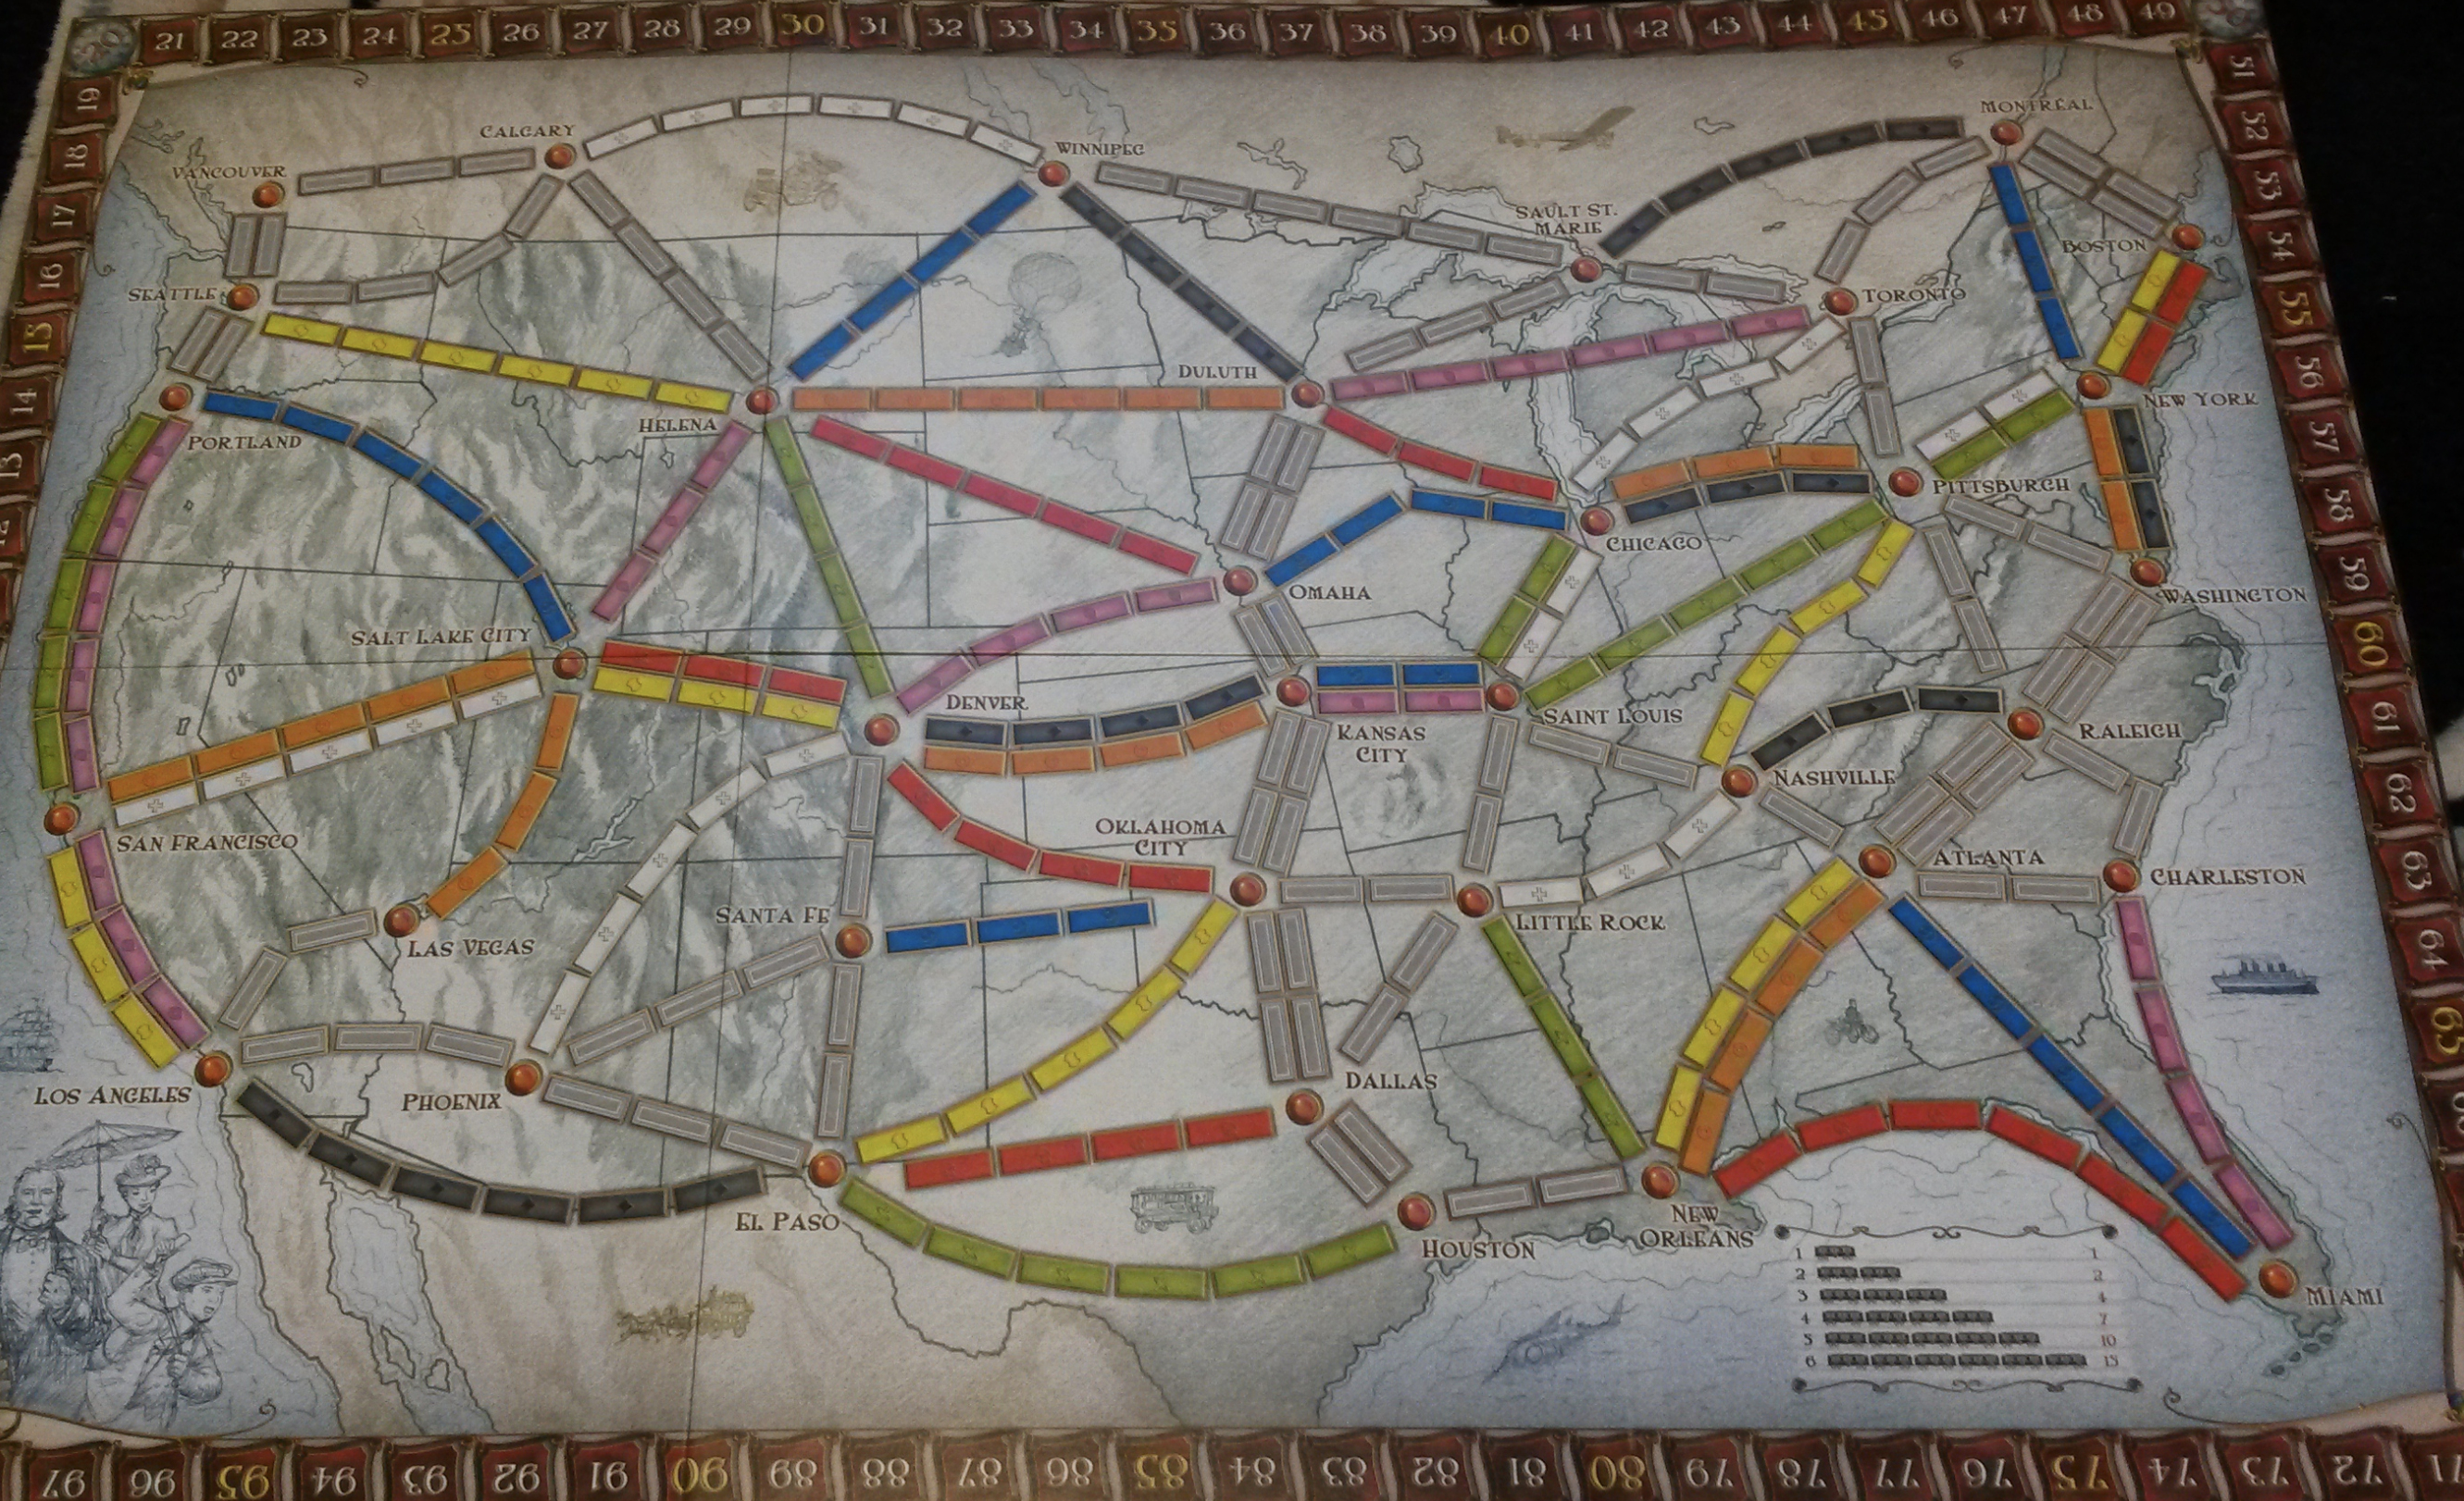
\includegraphics[scale=.3]{figures/board}
\end{frame}

\begin{frame}{Overview}
    Routes
    \begin{itemize}
        \item Long routes are overvalued ... and can 
        be used to easily win.
        \item We can find a better route scoring scheme 
        with indicator random variables.
    \end{itemize}
    
    Destination Tickets
    \begin{itemize}
        \item Players with some Destination Tickets perform
        better than players with others ... why?
        \item We use regression to identify
        the best Destination Tickets.
    \end{itemize}
    
\end{frame}

\section{Routes}

\begin{frame}{Current Route Values}
    \begin{center}
    %\renewcommand{\arraystretch}{2}
    \begin{tabular}{| c | c | c | c | c | c | c |}
    \hline
     Route Length & 1 & 2 & 3 & 4 & 5 & 6\\
     \hline
     Points Scored & 1 & 2 & 4 & 7 & 10 & 15\\
     \hline
     Points per Train & 1.00 & 1.00 & $1.\overline{33}$ 
     & 1.75 & 2.00 & 2.50\\
     \hline
    \end{tabular}
    \end{center}
    \pause
    Arguments for
    \begin{itemize}
        \item Collecting many trains of the same color is hard
    \end{itemize}
    Arguments against
    \begin{itemize}
        \item Is it really \textit{that} hard?
        \item Only one route can be claimed per turn
        \item Collecting multiple colors simultaneously helps
    \end{itemize}
\end{frame}

\begin{frame}{Games with routes of length at most $k$}
    For all games, all 45 trains will be collected over 23 turns.\footnotemark[2]
    
    \vspace{.5cm}
    \renewcommand{\arraystretch}{1.5}
    \begin{tabular}{| c | c | c | c | c |}
    \hline
    $k$ & Composition & Points & Turns & Points per Turn\\
    \hline
    1 & 1 x 45 & 45 & 23 + 45 & 0.66\\
    \hline
    2 & 2 x 22, 1 x 1 & 45 & 23 + 23 & 0.98\\
    \hline
    3 & 3 x 15 & 60 & 23 + 15 & 1.58\\
    \hline
    4 & 4 x 11, 1 x 1 & 78 & 23 + 12 & 2.23\\
    \hline
    5 & 5 x 9 & 90 & 23 + 9 & 2.81\\
    \hline
    6 & 6 x 7, 3 x 1 & 109 & 23 + 8 & 3.52\\
    \hline
    \end{tabular}
    \footnotetext[2]{We ignore locomotives collected
    from the five face up cards.}
\end{frame}

\begin{frame}{Win Rate in Simulated Games}
    \centering
    \includegraphics[scale=.45]{"figures/win_rates"}
\end{frame}

\begin{frame}{How \textit{should} routes be valued?}
   Idea:
   \vspace{1cm}
   value = expected time to collect \footnotemark[3]
   \footnotetext[3]{measured in number of cards
   rather than turns}
\end{frame}

\begin{frame}{Expected number to find $k$ blue cards}
   \only<1>{
   Without loss of generality, our goal is to
   calculate the expected numbers to find
   $k$ blue cards.
   }
   \only<2>{
   \begin{align}
    N_k&:= \text{number of cards until 
    $k$ blue cards are found} \nonumber \\
    C&:= \text{all cards} \nonumber \\
    B&:= \text{blue cards} \nonumber \\
    x &\in C \setminus B \nonumber \\
    I_{x,k}&:= 
    \begin{cases} 
      1 & \text{if $x$ appears before 
      the $k^{th}$ blue card} \\
      0 & \text{otherwise}
   \end{cases}
   \nonumber
   \end{align}
    Then
    \begin{align}
        N_k = k + \sum_{x \in C \setminus B} I_{x,k} \nonumber
    \end{align}
   }
   \only<3>{
    \begin{align}
        N_k = k + \sum_{x \in C \setminus B} I_{x,k} \nonumber
    \end{align}
   Taking expectation,
   \begin{align}
       \E[N_k] = k + 
       \left ( |C \setminus B| \right) \times
       \E[I_{x,k}] \nonumber
   \end{align}
   Recall $\E[I_{x,k}] = 1 \times \p(I_{x,k}=1) +
   0 = \p(I_{x,k}=1)$.
   
   \vspace{.5cm}
   Then
    \begin{align}
       \E[N_k] = k + 
       \left ( |C \setminus B| \right) \times
       \p(I_{x,k}=1) \nonumber
   \end{align}  
   }
   \only<4>{
   Think of the deck as non-blue cards separated by blue cards
   into $|B| + 1$ piles (possibly of size 0):
   \begin{align}
       xxxbxbbxxxbxbb\dots xbxxxb \nonumber
   \end{align}
   Then $\p(I_{x,k}=1)$ is $k/(|B| + 1)$
   }
   \only<5>{
    \begin{align}
       \E[N_k] &= k + 
       \left ( |C \setminus B| \right) \times
       \frac{k}{|B| + 1} \nonumber \\
       &= \left(1 + \frac{110-12}{12+1} \right) k \nonumber\\ 
       &= \frac{111}{13} k \nonumber
   \end{align}
   Thus our scoring should be linear!!
   }
\end{frame}

\begin{frame}{Choosing a scalar}
    \centering
    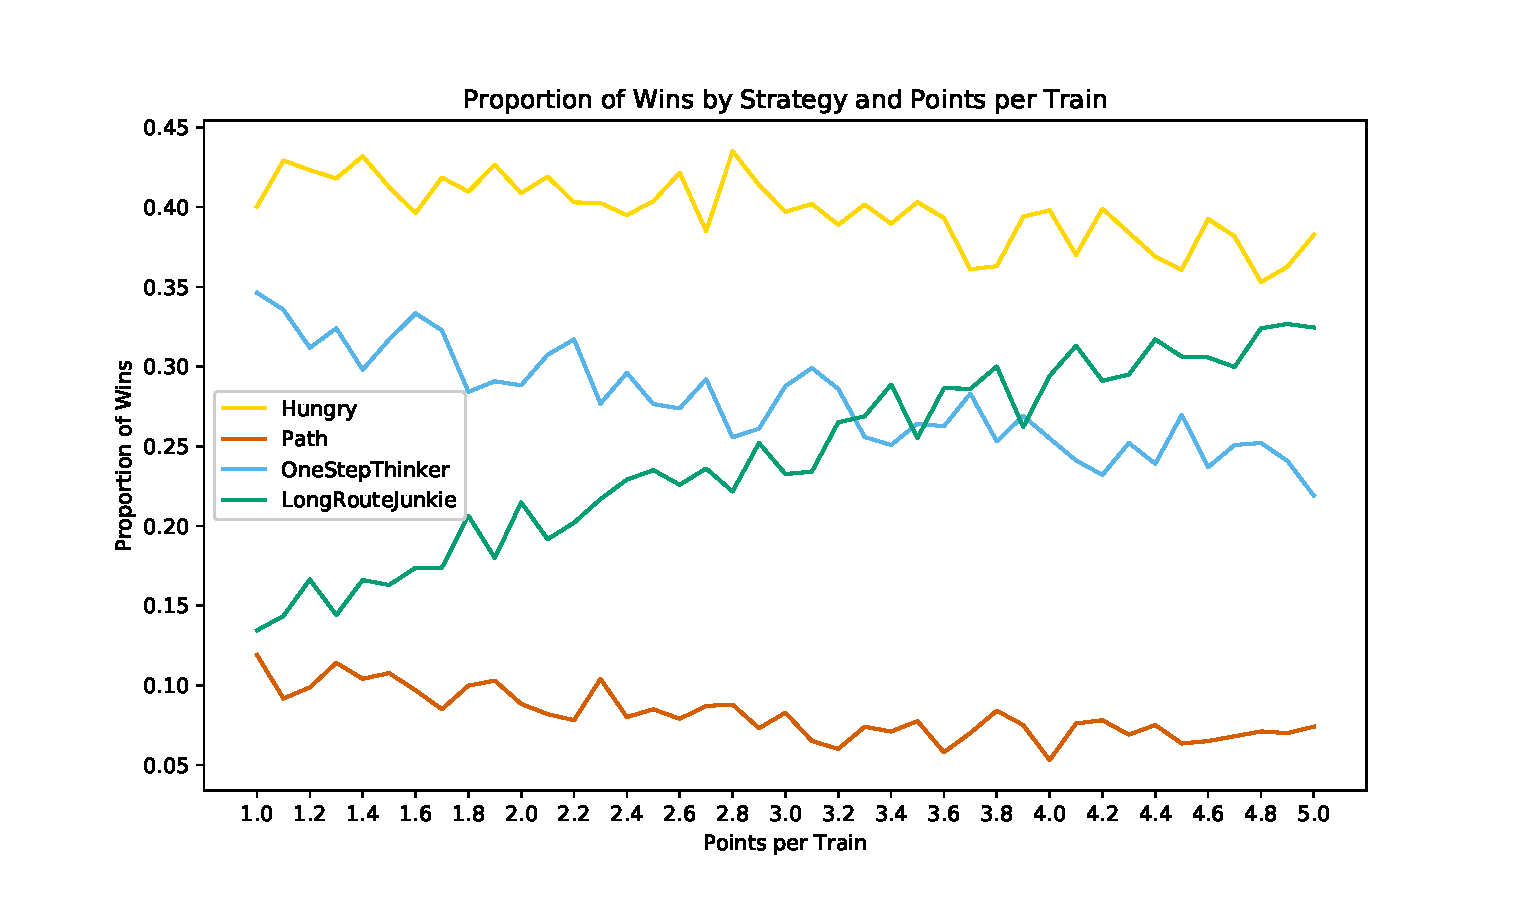
\includegraphics[scale=.45]{figures/points}   
    Perhaps somewhere between 3.5 and 5?
\end{frame}

\section{Destination Tickets}

\begin{frame}{Destination Tickets and Wins}
    \centering
    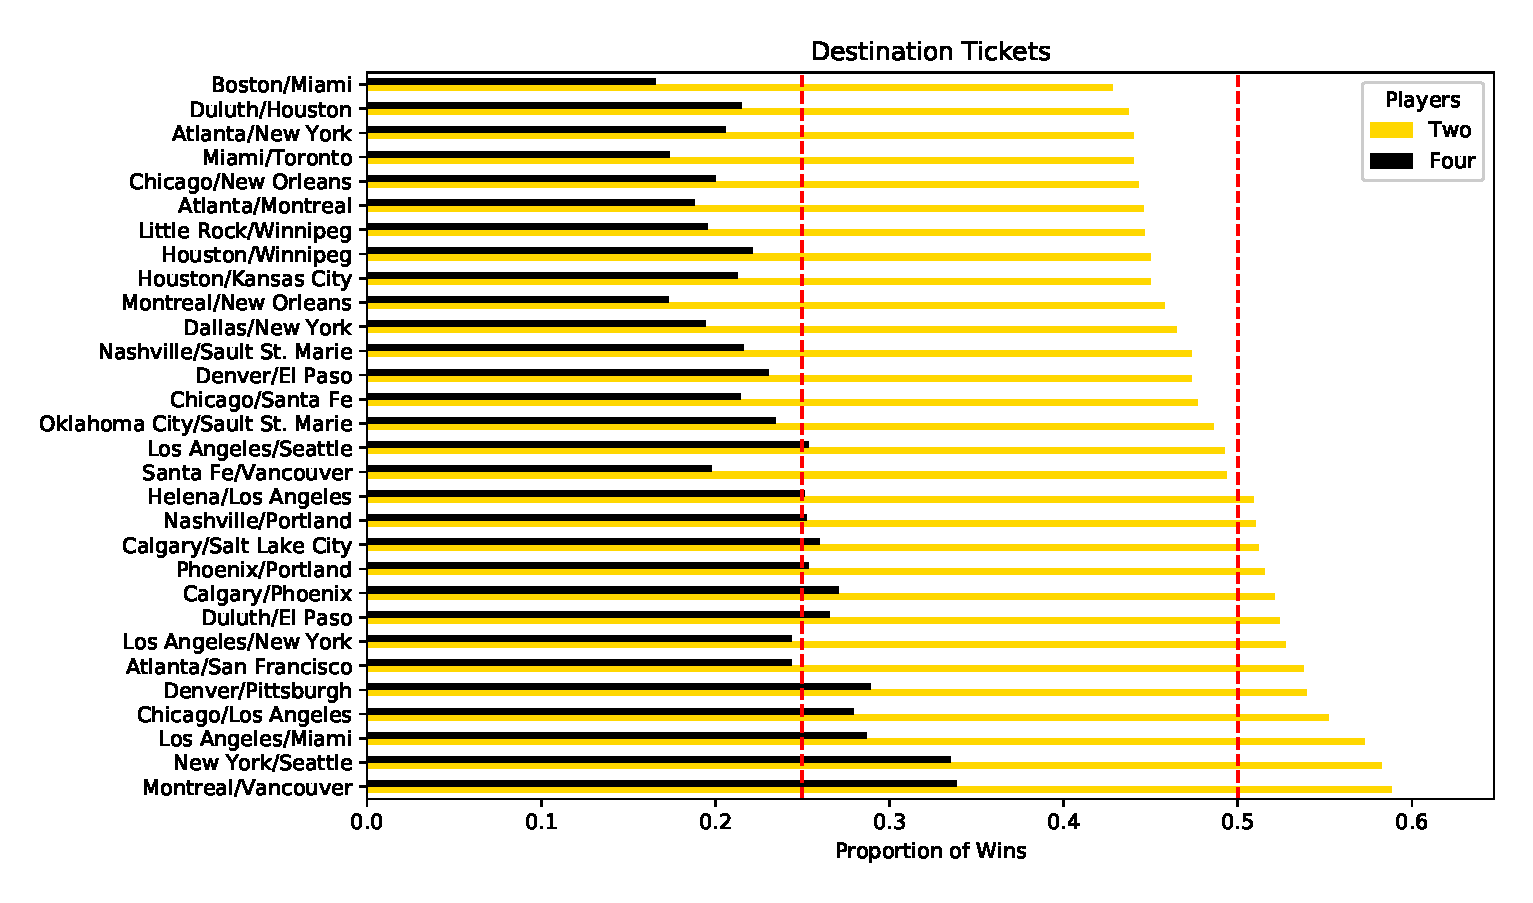
\includegraphics[scale=.45]{figures/destination_tickets}
\end{frame}

\begin{frame}{Best and Worst}
    Best: Montreal/Vancouver, New York/Seattle
    \begin{center}
    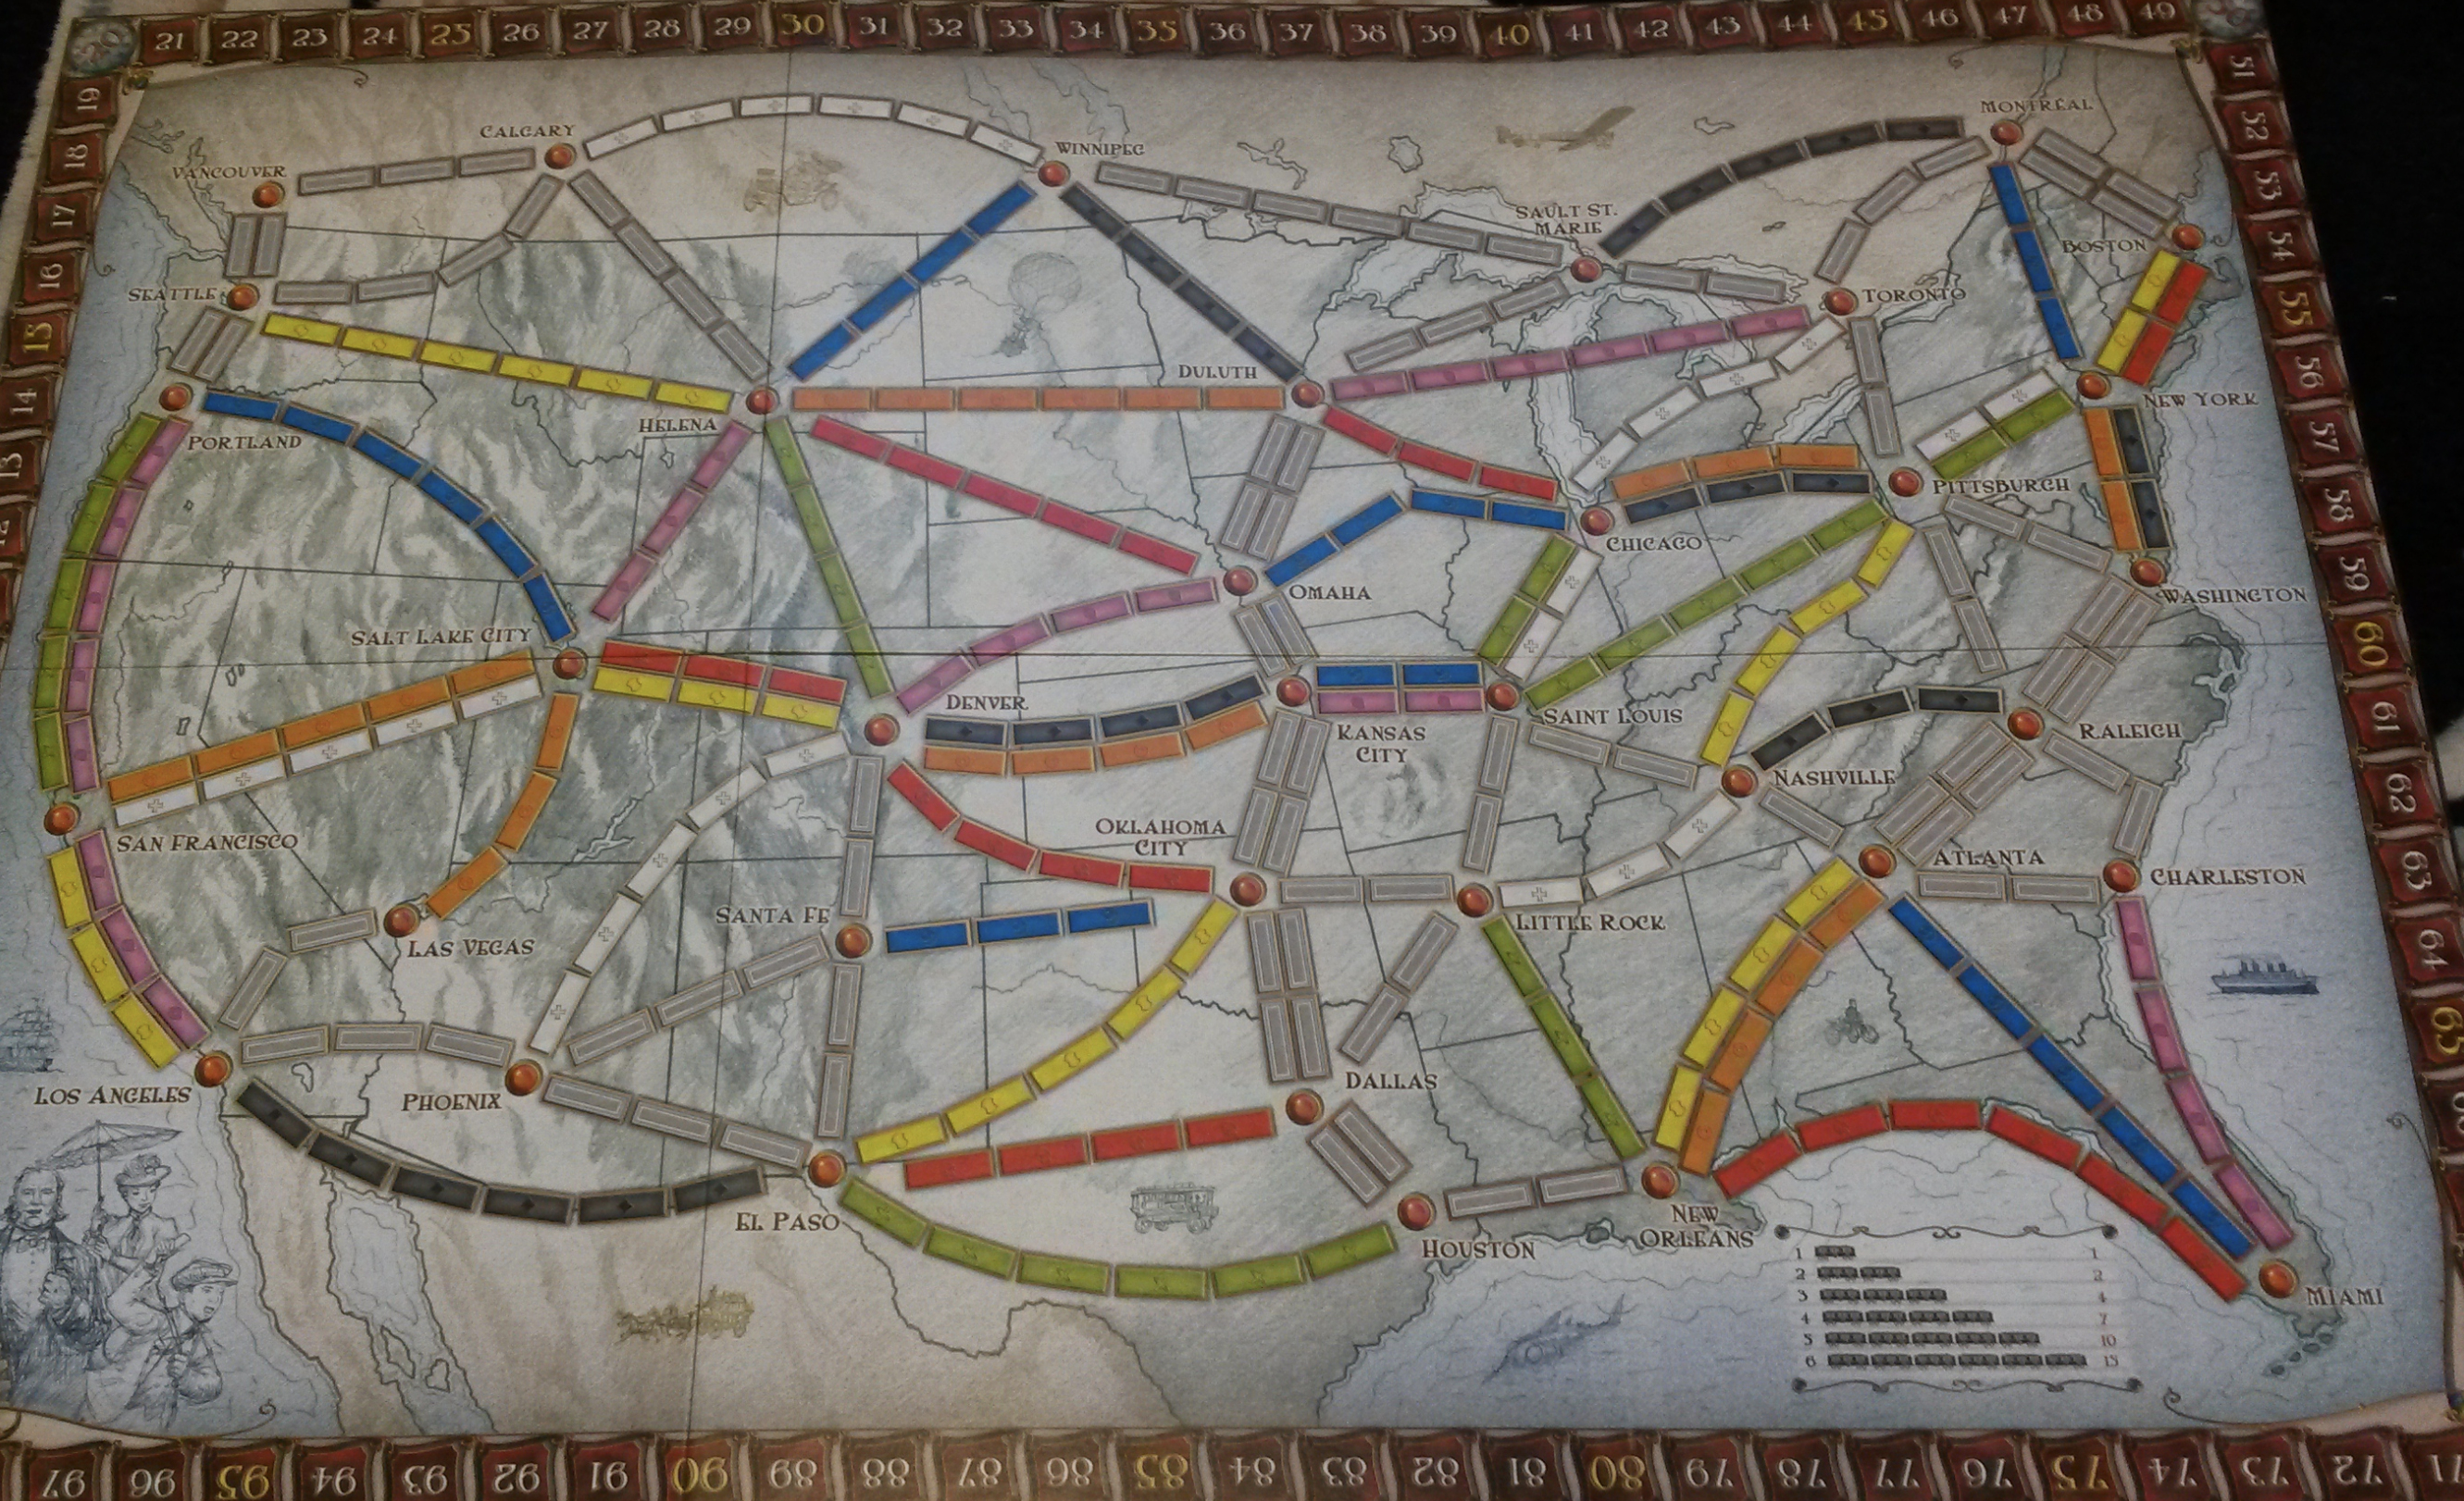
\includegraphics[scale=.25]{figures/board}
    \end{center}
    Worst: Boston/Miami
\end{frame}

\begin{frame}{Effective Resistance?}
    A measure of connectivity between two nodes on a graph:
    electric flow from one node to another
    \begin{align}
        \text{resistance} =
        \min_{\text{flows}}
        \sum_{\text{routes}}
        (\text{flow on route})^2
        \nonumber
    \end{align}
    
    More, shorter paths $\rightarrow$ lower resistance

\end{frame}

\begin{frame}{Effective Resistance!}
    \centering
    \includegraphics[scale=.45]{figures/resistance_aggregate}
\end{frame}

\begin{frame}{Rankings by Minimum Path Length and Residual}
    \centering
    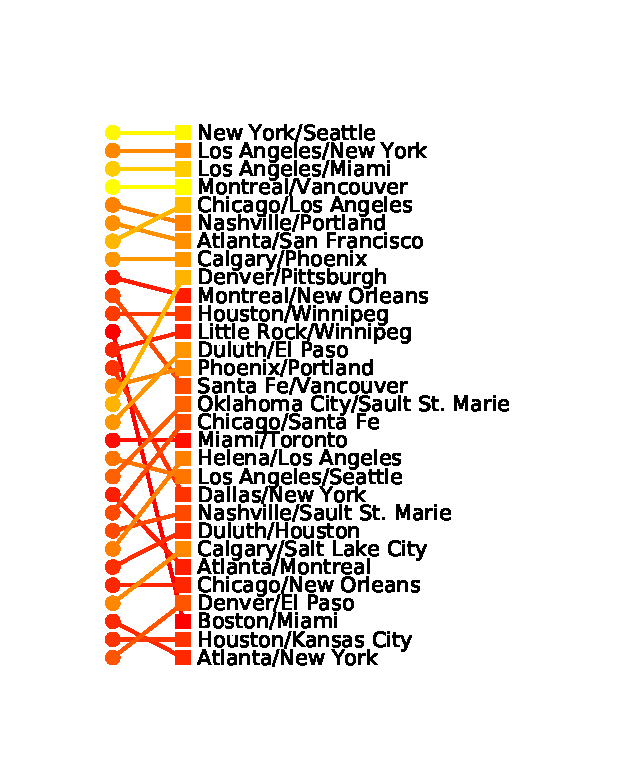
\includegraphics[scale=.2]{figures/rankings}
\end{frame}

\begin{frame}{Summary}
    Routes
    \begin{itemize}
        \item Long routes are overvalued ... and can 
        be used to easily win.
        \item We can find a better route scoring scheme 
        with indicator random variables.
    \end{itemize}
    
    Destination Tickets
    \begin{itemize}
        \item Players with some Destination Tickets perform
        better than players with others ... why?
        \item We use regression to identify
        the best Destination Tickets.
    \end{itemize}
    
\end{frame}

\begin{frame}{Thank you!}
    Questions?
\end{frame}

\begin{frame}{Correlations with overall wins}
   \begin{figure}
    \centering
    \begin{subfigure}
        \centering
        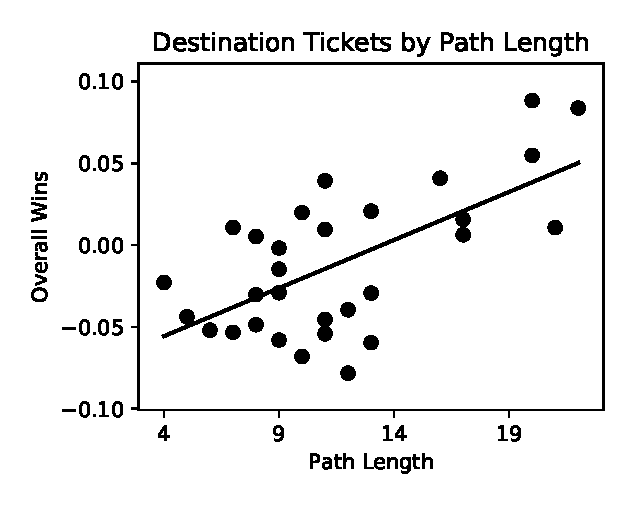
\includegraphics[height=1.3in]{figures/correlation0}
    \end{subfigure}
    \begin{subfigure}
        \centering
        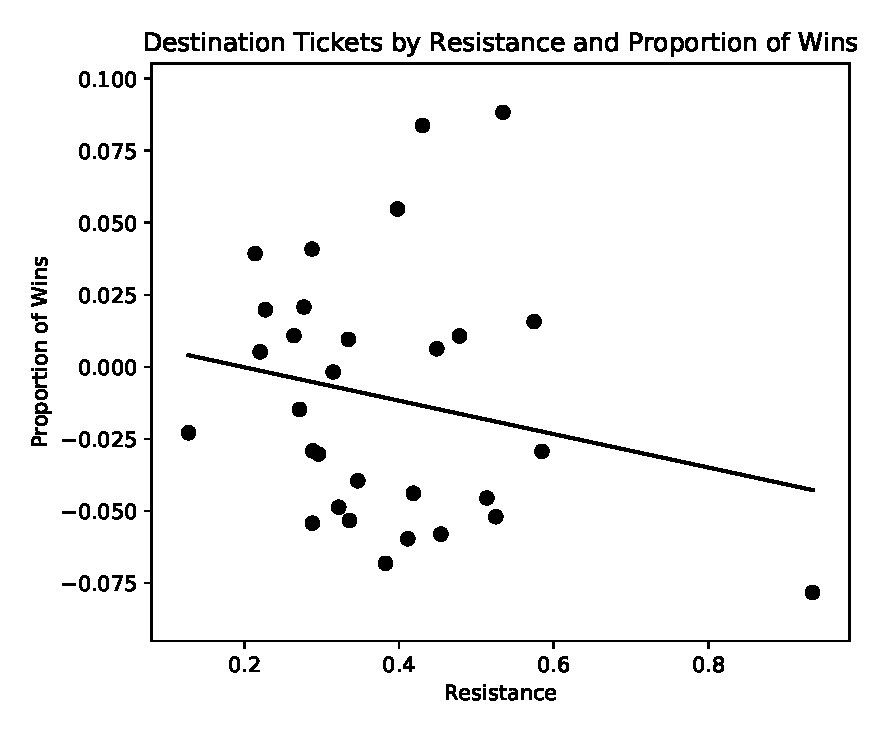
\includegraphics[height=1.3in]{figures/correlation1}
    \end{subfigure}
    \begin{subfigure}
        \centering
        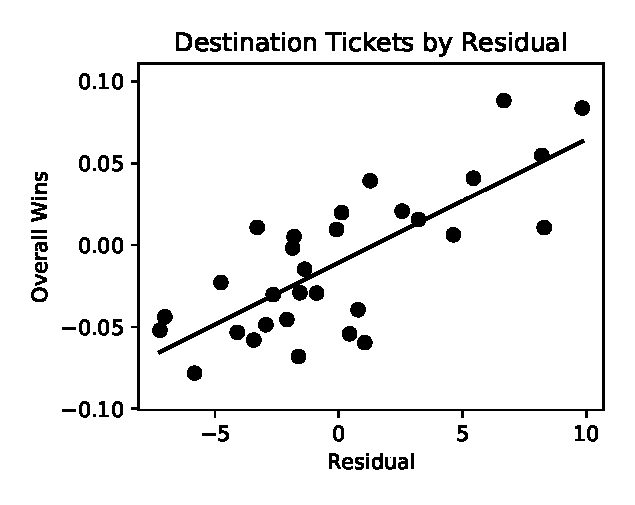
\includegraphics[height=1.3in]{figures/correlation2}
    \end{subfigure}
    \end{figure} 
\end{frame}

\begin{frame}{References}
    W. Ellens, F. Spieksma, P. Van Mieghem, 
    A. Jamakovic, and R. Kooij.
    Effective Graph Resistance. Linear Algebra and
    its Applications,435(10):2491–2506, 2011.
    
    \vspace{.5cm}
    F. de Mesentier Silva, S. Lee, J. Togelius, and A. Nealen.
    Ai-based Playtesting of Contemporary Board Games.
    In Proceedings ofthe 12th International Conference on the
    Foundations of Digital Games, page 13.  ACM, 2017
    
    \vspace{.5cm}   
    A. Moon.
    Ticket to Ride. [Board Game].
    \textit{Days of Wonder: Los Altos, CA}, 2004
\end{frame}

\end{document}